\documentclass[14pt]{beamer}
\title{OTHELLO}
\date{21-10-2021}
\author[Bvrith]{RICHA CRISTINA: 20WH1A0576: CSE  \\  P MEGHANA: 20WH1A12A8: IT \\ K SUSHMEETHA: 20WH1A1258: IT \\ G ALEKHYA: 20WH1A0432: ECE \\ P ARUNA: 20WH1A0237: EEE \\ BUSHRA: 21WH1A0204:  EEE }

\usefonttheme{serif}
\usepackage{bookman}
\usepackage{hyperref}
\usepackage[T1]{fontenc}
\usepackage{graphicx}
\usecolortheme{orchid}
\beamertemplateballitem

\begin{document}
    \begin{frame}
        \titlepage
	\small{BVRIT Hyderabad College of Engineering for Women}
    \end{frame}
    \begin{frame}
	\frametitle{Introduction}
        \begin{itemize}
	       \item Othello is a game played by two people on an 8 x 8 board.
            \item One player places disks with the white side up and the other with black side up.
            \item The players alternate placing one disk on an unoccupied space on the board.
	\end{itemize}
    \end{frame}

    \begin{frame}
	    \frametitle{Approach}
	\begin{itemize}
	    \item We intend to approach the problem statement by using pygame and tkinter.
	\end{itemize}
    \end{frame}


    \begin{frame}
        \frametitle{Challenges}
	\begin{itemize}
	    \item Gathering information
          \item Preparing the repository
          \item Installing the software needed
	\end{itemize}
    \end{frame}
    \begin{frame}
	\frametitle{Learning}
        \begin{itemize}
	    \item Tkinter and Pygame
        \end{itemize}
    \end{frame}

    \begin{frame}
	\frametitle{GIT}
         \begin{figure}
	          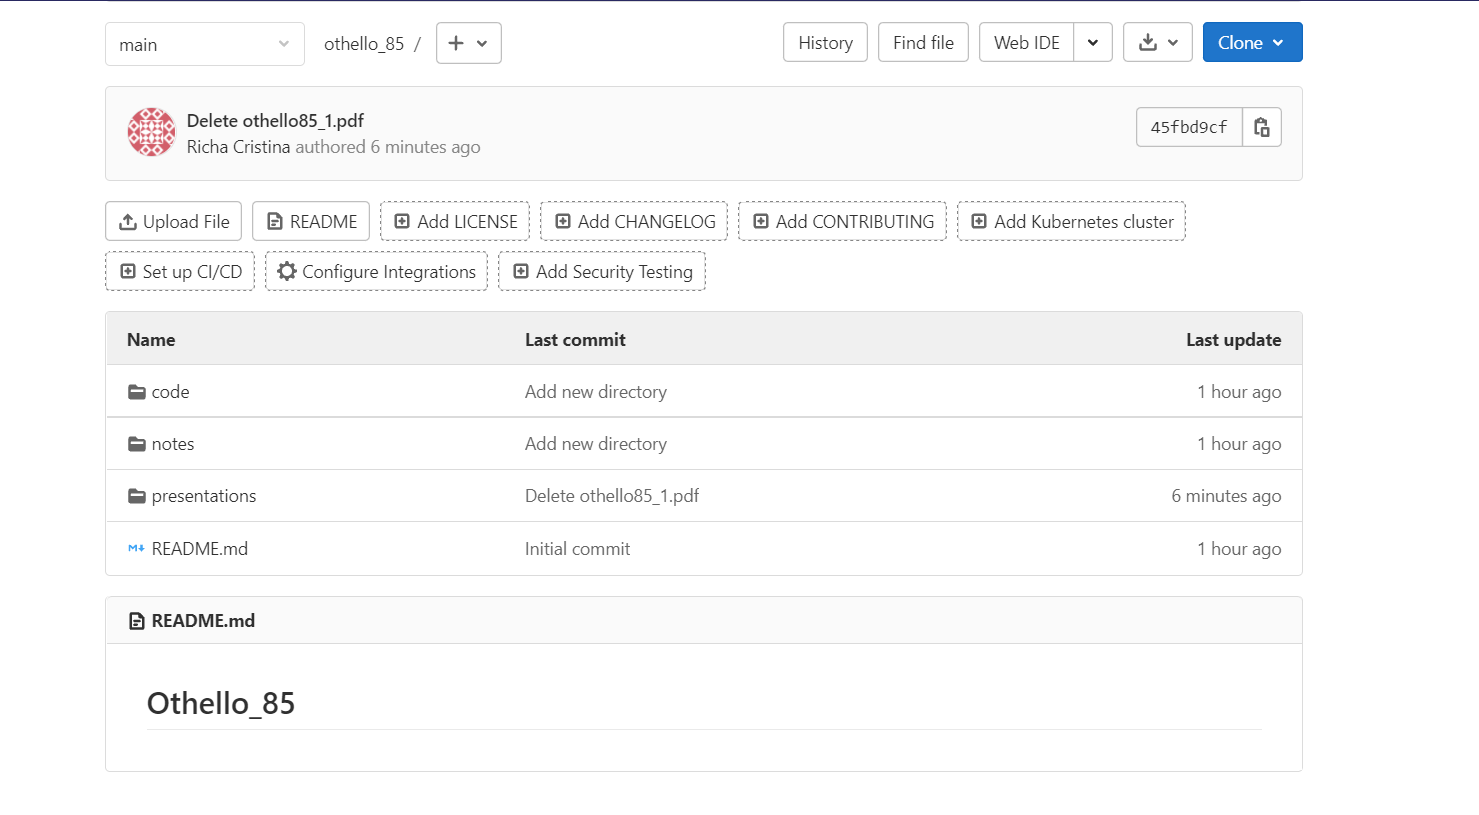
\includegraphics [width = 10cm] {repository.png}
          \end {figure}
    \end{frame}
   
   
    \begin{frame}
	\begin{center}
	     THANK YOU!!!
	\end{center}
    \end{frame}
\end{document}
